
\documentclass[11pt]{article}
\usepackage{amsmath, amssymb, graphicx, outline, float, cite, color}
\usepackage{lineno}

%%%%%%%%%%%%%%%%%%%%%%%%%%%%%%%%%%%%%%%%%
% Wenneker Article
% Structure Specification File
% Version 1.0 (28/2/17)
%
% This file originates from:
% http://www.LaTeXTemplates.com
%
% Authors:
% Frits Wenneker
% Vel (vel@LaTeXTemplates.com)
%
% License:
% CC BY-NC-SA 3.0 (http://creativecommons.org/licenses/by-nc-sa/3.0/)
%
%%%%%%%%%%%%%%%%%%%%%%%%%%%%%%%%%%%%%%%%%

%----------------------------------------------------------------------------------------
%	PACKAGES AND OTHER DOCUMENT CONFIGURATIONS
%----------------------------------------------------------------------------------------

\usepackage[english]{babel} % English language hyphenation

\usepackage{microtype} % Better typography

\usepackage{amsmath,amsfonts,amsthm} % Math packages for equations

\usepackage[svgnames]{xcolor} % Enabling colors by their 'svgnames'

\usepackage[hang, small, labelfont=bf, up, textfont=it]{caption} % Custom captions under/above tables and figures

\usepackage{booktabs} % Horizontal rules in tables

\usepackage{lastpage} % Used to determine the number of pages in the document (for "Page X of Total")

\usepackage{graphicx} % Required for adding images

\usepackage{enumitem} % Required for customising lists
\setlist{noitemsep} % Remove spacing between bullet/numbered list elements

\usepackage{sectsty} % Enables custom section titles
\allsectionsfont{\usefont{OT1}{phv}{b}{n}} % Change the font of all section commands (Helvetica)

%----------------------------------------------------------------------------------------
%	MARGINS AND SPACING
%----------------------------------------------------------------------------------------

\usepackage{geometry} % Required for adjusting page dimensions

\geometry{
	top=2cm, % Top margin
	bottom=2cm, % Bottom margin
	left=3cm, % Left margin
	right=3cm, % Right margin
	includehead, % Include space for a header
	includefoot, % Include space for a footer
	%showframe, % Uncomment to show how the type block is set on the page
}

\setlength{\columnsep}{7mm} % Column separation width

%----------------------------------------------------------------------------------------
%	FONTS
%----------------------------------------------------------------------------------------

\usepackage[T1]{fontenc} % Output font encoding for international characters
\usepackage[utf8]{inputenc} % Required for inputting international characters

\usepackage{XCharter} % Use the XCharter font

%----------------------------------------------------------------------------------------
%	HEADERS AND FOOTERS
%----------------------------------------------------------------------------------------

\usepackage{fancyhdr} % Needed to define custom headers/footers
\pagestyle{fancy} % Enables the custom headers/footers

\renewcommand{\headrulewidth}{0.0pt} % No header rule
\renewcommand{\footrulewidth}{0.4pt} % Thin footer rule

\renewcommand{\sectionmark}[1]{\markboth{#1}{}} % Removes the section number from the header when \leftmark is used

%\nouppercase\leftmark % Add this to one of the lines below if you want a section title in the header/footer

% Headers
\lhead{} % Left header
\chead{\textit{\thetitle}} % Center header - currently printing the article title
\rhead{} % Right header

% Footers
\lfoot{} % Left footer
\cfoot{} % Center footer
\rfoot{\footnotesize Page \thepage\ of \pageref{LastPage}} % Right footer, "Page 1 of 2"

\fancypagestyle{firstpage}{ % Page style for the first page with the title
	\fancyhf{}
	\renewcommand{\footrulewidth}{0pt} % Suppress footer rule
}

%----------------------------------------------------------------------------------------
%	TITLE SECTION
%----------------------------------------------------------------------------------------

\newcommand{\authorstyle}[1]{{\large\usefont{OT1}{phv}{b}{n}\color{DarkRed}#1}} % Authors style (Helvetica)

\newcommand{\institution}[1]{{\footnotesize\usefont{OT1}{phv}{m}{sl}\color{Black}#1}} % Institutions style (Helvetica)

\usepackage{titling} % Allows custom title configuration


%\newcommand{\HorRule}{\color{DarkGrey}\rule{\linewidth}{1pt}} % Defines the gold horizontal rule
\newcommand{\HorRule}{\color{DarkGoldenrod}\rule{\linewidth}{1pt}} % Defines the gold horizontal rule
 
\pretitle{
	\vspace{-30pt} % Move the entire title section up
	\HorRule\vspace{10pt} % Horizontal rule before the title
	\fontsize{20}{18}\usefont{OT1}{phv}{b}{n}\selectfont % Helvetica
	\color{DarkRed} % Text colour for the title and author(s)
}

\posttitle{\par\vskip 15pt} % Whitespace under the title

\preauthor{} % Anything that will appear before \author is printed

\postauthor{ % Anything that will appear after \author is printed
	\vspace{10pt} % Space before the rule
	\par\HorRule % Horizontal rule after the title
	\vspace{20pt} % Space after the title section
}

%----------------------------------------------------------------------------------------
%	ABSTRACT
%----------------------------------------------------------------------------------------

\usepackage{lettrine} % Package to accentuate the first letter of the text (lettrine)
\usepackage{fix-cm}	% Fixes the height of the lettrine

\newcommand{\initial}[1]{ % Defines the command and style for the lettrine
	\lettrine[lines=3,findent=4pt,nindent=0pt]{% Lettrine takes up 3 lines, the text to the right of it is indented 4pt and further indenting of lines 2+ is stopped
		%\color{DarkRed}% Lettrine colour
		\color{DarkGoldenrod}% Lettrine colour
		{#1}% The letter
	}{}%
}

\usepackage{xstring} % Required for string manipulation

\newcommand{\lettrineabstract}[1]{
	\StrLeft{#1}{1}[\firstletter] % Capture the first letter of the abstract for the lettrine
	\initial{\firstletter}\textbf{\StrGobbleLeft{#1}{1}} % Print the abstract with the first letter as a lettrine and the rest in bold
}

%----------------------------------------------------------------------------------------
%	BIBLIOGRAPHY
%----------------------------------------------------------------------------------------

%\usepackage[backend=bibtex,style=authoryear,natbib=true]{biblatex} % Use the bibtex backend with the authoryear citation style (which resembles APA)

%\addbibresource{example.bib} % The filename of the bibliography

%\usepackage[autostyle=true]{csquotes} % Required to generate language-dependent quotes in the bibliography



\graphicspath{ {Figs/} }

\usepackage[normalem]{ulem}
\usepackage[T1]{fontenc}
\usepackage[utf8]{inputenc}
\usepackage{authblk}
\usepackage{framed}

\newcommand{\tcr} { \textcolor{red} }
\newcommand{\tcb} { \textcolor{blue} }


\title{
Modeling the effects of the immune system and EMT on epithelial cancer progression
}

\author{ Daniel R. Bergman\textsuperscript{1},
Matthew K. Karikomi\textsuperscript{1},
Min Yu\textsuperscript{4},
Qing Nie\textsuperscript{1,2,*},
and Adam L. MacLean\textsuperscript{1,3,*}
\newline\newline % Space before institutions
	\textsuperscript{1}Department of Mathematics, University of California, Irvine,  Irvine, CA 92697 \\
        \textsuperscript{2}Department of Cell and Developmental Biology, University of California, Irvine, Irvine, CA 92697 \\
        \textsuperscript{3}Department of Biological Sciences, University of Southern California, Los Angeles, CA 90089 \\
        \textsuperscript{4}Department of Stem Cell \& Regenerative Medicine, Keck School of Medicine, University of Southern California, Los Angeles, CA 90033 \\
        \textsuperscript{*}Correspondence:  qnie@uci.edu (Q.N.); macleana@usc.edu (A.L.M.). }

\renewcommand\Authands{ and }

\date{}


\begin{document}
\maketitle

\thispagestyle{firstpage} % Apply the page style for the first page (no headers and footers)


%\section*{Abstract}
\lettrineabstract{During progression from carcinoma in situ to an invasive tumor, the immune system is engaged in complex sets of interactions with various tumor cells. Moreover, tumor cell plasticity can significantly alter disease trajectories via epithelial-to-mesenchymal transition (EMT). Several of the same pathways that regulate EMT are involved in tumor-immune interactions, yet little is known about the mechanisms and consequences of crosstalk between these regulatory processes. Here we introduce a multiscale evolutionary model to describe  tumor-immune-EMT interactions and their impact on epithelial cancer progression from in situ to invasive disease. Through in silico analyses of large patient cohorts, we find controllable regimes that maximize invasion-free survival. We identify that delaying tumor progression depends crucially on properties of the mesenchymal tumor cell phenotype: its growth rate and its immune-evasiveness. Through analysis of inflammation-associated cancer data from The Cancer Genome Atlas, we find that -- in agreement with model predictions -- association with EMT significantly worsens invasion-free survival probabilities. These results offer novel means to delay disease progression by regulating properties of EMT, and demonstrate the importance of studying cancer-immune interactions in light of EMT.
}


\linenumbers


%%%%%%%%%%%%%%%%%%%%%%%%%%%%%%%%%%%%%
     %                    INTRODUCTION                    %
%%%%%%%%%%%%%%%%%%%%%%%%%%%%%%%%%%%%%

\section{Introduction}
The majority of deaths from cancer are due to metastasis of the disease \cite{dillekaas201990}. It is thus of critical importance to understand better the progression from in situ to invasive disease. Underlying this progression are genetic and epigenetic events, including mutations in pathways critical to the success of the cancer cell (driver mutations) \cite{ryan2016hallmarks}. These pathways include cell proliferation, apoptosis, and immunogenicity.
\par 
Cancer and the immune system interact in myriad ways. The immune system modulates the tumor microenvironment (TME), since immune signals that affect the tumor can be amplified or repressed through feedback in response to local inflammatory signals. This complex cell signaling occurs alongside the targeting (and potential eradication) of the tumor by immune cells \cite{de2006paradoxical}.
\par 
The effects of the immune system on a tumor can be broadly summarized into two branches. The cytotoxic branch of the immune system, such as natural killer cells (NKs) and cytotoxic T cells (CTLs), seek out and lyse tumor cells. Upon carrying out their effector functions, these cytotoxic cells lose efficacy or deactivate \cite{finn12_immunooncology-1}. The regulatory branch of the immune system (Tregs, and other factors), inhibits the effective functioning of the cytotoxic branch \cite{ruffell2010lymphocytes}.
Inflammation can increase the probability of cancer incidence and progression, with some of the most pronounced effects seen for tumors originating in gastrointestinal and pancreatic tissues \cite{hu10_inflammationinduced, balkwill01_inflammation}.
Recent work has shown, contrary to the typical effects of inflammation on cancer, that under certain conditions inflammation may not be oncogenic but rather onco-protective \cite{guo17_multiscale}.
\par
Immunotherapies are beginning to realize their potential, with significant impacts on patient health and survival \cite{pardoll2012blockade,restifo2012adoptive}, and may even provide a cure for certain hematopoietic cancers via anti-CD19 CAR-T cells \cite{safeandpotent}. The presentation of antigens on tumor cells is recognized by innate immune cells that are transported to lymph nodes where T cells (and other components) can be activated \cite{schreiber11_cancer}.
The tumor also engages in processes that can indirectly modify the TME, for example by releasing transforming growth factor beta (TGF-$\beta$), which can shif the TME towards a tumor-supportive environment by enhancing immunosuppression via activation of Tregs \cite{schreiber11_cancer}.
\par
Epithelial-to-mesenchymal transition (EMT) describes a reversible process by which cells displaying an epithelial phenotype transition into cells with a mesenchymal phenotype.
Epithelial cells are -- in part -- defined by tight cell-cell adhesion. Mesenchymal cells exhibit less adhesion, greater ranges of motility, and may possess stem-like properties \cite{nieto2016emt}, although controversy regarding `stemness' and EMT remains \cite{nie18_stem, sha19_intermediate}.  
Recent work has shown that -- rather than being a binary process -- at least two stable intermediate EMT states exist \cite{hong2015ovol2, jolly15_coupling}.
Ongoing investigations into the plasticity and stability of EMT overlap with discussions elsewhere, e.g. of discrete vs. continuous processes during cell differentiation \cite{moris16_transition}.
Intermediate states have emerged as a central mechanism by which cell fates (and the noise inherent within them) can be controlled \cite{maclean18_exploring, ta16_controlling, rackauckas18_meanindependent}. 
\par 
Two features of the mesenchymal phenotype are of particular relevance in the context of cancer-immune interactions. i) mesenchymal tumor cells proliferate less than epithelial cells, we refer to this as mesenchymal growth arrest (MGA), and can be considered related to (in the sense of quiescence) the ``stemness'' phenotype of the mesenchymal tumor cells \cite{woods2014effects}. ii) mesenchymal cells are less susceptible to immune clearance \cite{terry2017new}. As a cell is targeted by cytotoxic immune cells for clearance, a physical connection between the two cells must be established. This immunological synapse -- mediated in part by T-cell receptors bound to antigens and the major histocompatibility complex on the target cell -- is down-regulated in mesenchymal cells, thus inhibiting formation of the synapse \cite{terry2017new}. We refer to this phenotype as mesenchymal immune evasion (MIE).
\par
In addition to the prominent role it plays in metastasis, EMT has more recently been shown to also regulate other aspects of tumor progression \cite{nieto2016emt,peinado2007snail}.
TGF-$\beta$, a master regulator of EMT \cite{lim2012epithelial}, is at once implicated heavily in tumor-mediated immune responses, since Tregs release TGF-$\beta$ upon arriving at the tumor site\cite{terry2017new}. In hepatocellular carcinoma, for example, there is direct evidence linking Treg-secreted TGF-$\beta$ with EMT \cite{shi2019cd4+}. Thus, even by considering only the TGF-$\beta$ pathway, we find compelling evidence that  these three core components (the tumor, the immune system, and EMT) all interact. It therefore strikes us as a priority to develop models to understand how the interactions between each of these three components affect cancer incidence and progression.
\par
%The other facet of mesenchymal cells is their slower proliferation rate, and this is tied to the observation that mesenchymal cells have been speculated to exhibit a more ``stemness'' phenotype. While many cell behaviors are associated with stemness, here we target the specific reduction in proliferation rate \cite{woods2014effects}.
%Cancer cells are of course characterized by some degree of unregulated proliferation, thus it is appealing to explore the effects of differential proliferation rates within the cancer cell population.
%In our model, we refer to the reduced proliferative capacity associated with a mesenchymal cell phenotype as mesenchymal growth arrest (MGA).
\par
Mathematical oncology, that is, mathematical models of cancer incidence, progression, and treatment, has become a well-developed field; many models have offered insight into the cellular interactions underlying cancer and its interplay with the immune system, including older \cite{anderson98_continuous, sherrattjonathana.92_oncogenes, pillis05_validated} and more recent works \cite{kim18_cell, gallaher14_bridging, gallaher18_spatial, an15_agentbased, serre16_mathematical, louzoun14_mathematical, briones-orta13_arkadia, lavi13_role, greene15_modeling, greene16_mathematical, cho17_modeling-1,  benzekry17_mathematical, owen11_mathematical, west18_multidrug}. These studies have increased our understanding of how tumors grow in the presence of various immune components, and how treatment regimes can be designed to maximize the efficacy of cytotoxicity while minimizing risks to the patient. However, to our knowledge no models have addressed how the effects of EMT alter interactions between the immune system and cancer, and the subsequent implications for treatment. 
\par
Here we develop a model with the goal of studying interactions between the tumor, the immune system and EMT.
We seek to describe a set of crucial molecular and cellular interactions in epithelial tumor cells, including effects due to DNA damage and mutation, to investigate the probability that in situ tumors will progress and, if so, when.
A recent model of cancer-immune interactions \cite{guo17_multiscale} described the effects of the TME on the risk of cancer, and we build on the core cell cycle component of this model, adding significant new interactions to the immune component of the model (which was previously modeled by a single interaction), as well as adding the effects of EMT.
In doing so, we shift the focus of the previous model from cancer initiation to cancer progression.
We do this to reflect the fact that cancer progression hinges on escape from the immune system and the fact that EMT has a more well-defined role during progression and metastasis.
We seek to understand whether this more complex immune module will change our understanding of inflammatory effects on the tumor, and how the epithelial-mesenchymal axis influences these.
\par 
In the next section we develop the model, explaining the intuition behind each of its components.
We go on to analyze its behavior: global ``{\em one-at-a-time}'' sensitivity analysis identifies parameters that are crucial for progression.
We study these in more depth, focusing on the competing effects of EMT and of the immune system on progression, and discover that EMT intricately regulates progression: under certain regimes a careful balance of EMT- and immune-driven processes can significantly prolong invasion-free survival.
To test these predictions, we analyze data from the Cancer Genome Atlas (TCGA), and find evidence for the synergistic effects of inflammation and EMT predicted by the model for patients with pancreatic or ovarian cancer.



\begin{framed}
    {\bf Quick Guide to Equations and Assumptions}
    \newline
    To become invasive, An in situ tumor relies on mutations to alter cellular signaling pathways that enable cancer progression. The immune system simultaneously responds to the tumor upon recognition of neoantigens, and shapes the TME through dynamic inflammatory and regulatory signals.
\newline
% \hspace{50mm}
To capture these dynamics, we developed a non-spatial agent-based model. Tumor cells are modeled individually as agents and immune cell populations are described homogeneously by differential equations. We consider two tumor cell types: epithelial tumor cells (ETCs) and mesenchymal tumor cells (MTCs). Time is treated discretely in 18 hour steps; approximately the time of one cell cycle. During each cell cycle, tumor cells can either undergo division, apoptosis, immune clearance, or can rest. The likelihood that a cell will proliferate depends on the tumor size (competition for resources) and on cell-intrinsic factors. The likelihood that a cell will undergo apoptosis is constant but varies between cell types (ETC and MTC). The likelihood of immune clearance depends on the number and type of mutated cells in the tumor, cytotoxicity, regulatory cells, and cell-intrinsic factors.
\newline
As tumor cells proliferate, DNA damage can occur, and over time they become increasingly likely to acquire pathway mutations that change their propensities for proliferation or cell death. Natural killer (NK) cells identify and clear tumor cells, a process which results in neoantigens  priming and activating T cells in local lymph nodes. T cells can subsequently infiltrate the TME. At the tumor site, cytotoxic T cells (CTLs) lyse tumor cells, and T regulatory cells (Tregs) suppress cytotoxic activity. The following equation determine the per-cell cycle probability that a tumor cell will be lysed by a CTL:
    $$\rho_{\text{CTL}} =\delta_{\text{MUT}} \frac{N_{\text{CTL}}}{N_C/K_{1}+N_{\text{CTL}}}  \frac{E_{\text{CTL}}}{1+N_{\text{Treg}}/K_2} (1-\delta_{\text{IE}}\Delta_{\text{IE}})(1-\zeta \Delta_{\text{MIE}})$$
    Here, $\delta_\text{MUT}$ is 1 or 0 depending on whether or not the cell has a mutation. The second term is a hill function modeled after \cite{de2014modeling} and the third term describes onco-protective effects of Tregs. The second-to-last term describes the increased immune-evasiveness that can occur following mutation in the immune evasion pathway, and the last term quantifies the additional immune evasiveness of associated with MTCs. The inflammatory state of the TME thus impacts (through multiple factors) immune recruitment and cytotoxicity at the tumor site.
\newline
EMT impacts tumor cells through their proliferation and potential to evade the immune system change. MTCs have reduced proliferation %(by $\Delta_{MGA}$)
and increased immune evasiveness %(by $\Delta_{MIE}$).
%Cellular plasticity permits tumors cells by being able to undergo epithelial-to-mesenchymal transition (EMT) and move along this spectrum as a result of intrinsic and extrinsic factors.
%TGF-$\beta$, an activator of EMT, connects the tumor-immune model with EMT via its concentration in the TME.
TGF-$\beta$, an activator of EMT, is produced both by Tregs and tumor cells, thus connecting tumor-immune interactions with EMT, and as a result plays an important role in shaping tumor outcomes. EMT depends on TGF-$\beta$ concentration through a Hill-type function that determines the likelihood of EMT (or the reverse MET) through its magnitude relative to $\tau_{i-1}$. This is described by the equation:
    $$
    \tau_i = \frac{\tau_{\text{max}}}{N_C}\frac{\tau/K_3}{1+\tau/K_3} + X_i, \quad X_i \sim N(0,\sigma^2)
    $$
    Here, $\tau$ is the concentration of TGF-$\beta$ in the TME and $\tau_\text{max}$ represents a limit on the amount of TGF-$\beta$ that can be absorbed by all cells, with Gaussian noise added.
    \newline
    Our goal is to determine when the cancer becomes invasive, determined through the proportion of tumor cells harboring mutations in pathways that permit escape from in situ, relative to the total tumor cell population.
  \end{framed}




%%%%%%%%%%%%%%%%%%%%%%%
%                         METHODS                        %
%%%%%%%%%%%%%%%%%%%%%%%

%\begin{table}[H]
%\begin{tabular}{|p{\textwidth}|}
%\hline
%%%%
%\begin{itemize}
%\item TGF-$\beta$ is well-mixed within the TME
%\item All cells are on the same ``clock'', i.e. they all decide at the same time what to do next
%\item During a given cell cycle, exactly one event can happen to any one cell: proliferation, apoptosis, immune clearance, or rest
%\item All tumor cells (mutated and non-mutated) are equally likely to encounter immune cells
%\item Other spatial effects are ignored by the model, e.g. angiogenesis, hypoxia, invasive front, and chemotaxis
%\item The initial cells are mutated, but are not able to form an aggressive cancer without further mutations
%\end{itemize}
%\\
%\hline
%\end{tabular}
%\caption{Basic assumptions of the model}
%\label{table:model_assumptions}
%\end{table}


\section{Methods}
Here we briefly describe to core components of the model. Full details and equations are provided in the Supplement. We develop an agent-based model to describe the relationships between cancer, the immune system, and EMT, building on the cell-cycle and tissue-cell components described in \cite{guo17_multiscale}. 
The agents in the model are the cells that have already formed an in situ tumor yet lack key pathway mutations to become invasive.
In the process of the simulation, these cells can acquire mutations altering any of three key pathways (Fig. \ref{fig:ModelIntro}A).
%If the pathway is altered, the component is colored red and is marked with `X'.
%We distinguish between cells that have zero driver mutations and those with at least one as premalignant and malignant, respectively.
\par
We model immune cells as continuous variables, i.e. we assume that the tumor microenvironment is well-mixed with regards to the infiltrating immune cells.
The cytokine TGF-$\beta$ is also assumed to be well-mixed in the tumor microenvironment.
Tumor cells can take on either epithelial or mesenchymal phenotypes in a plastic manner: these phenotypes depend on both the TME and cell-intrinsic factors.
While the EMT score is continuous, a threshold determines if a given cell is labeled as epithelial or mesenchymal (Fig. \ref{fig:ModelIntro}).
%Even though each cell does have an EMT score on a spectrum of values, only the labeling influences its interactions in the model.

\subsection{Tumor evolution}\label{TissueCells}
Associated with each tumor cells are two essential features: their mutational signature and their EMT score. We consider three idealized pathways that can be mutated: proliferation, when altered this increases the probability of the cell proliferating within each cell cycle; apoptosis, when altered this decreases the probability of a cell undergoing apoptosis; and immune evasion, when altered this decreases the probability that a mutated cell will be cleared by immune components.
%The EMT score will be exposited in Section \ref{EMT}. 
 
\subsection{Immune population dynamics}\label{ImmuneSystem}
The immune system is modeled by three immune cell types: NKs, CTLs, and Tregs.
The NKs and CTLs act on the system by recognizing invasive cells and clearing them.
Upon clearance, they are deactivated and removed from the immune population.
Tregs suppress the function of NKs and CTLs (reduce tumor cell clearance), and in addition, release TGF-$\beta$ which further shapes the TME by pushing tissues cells more towards a mesenchymal phenotype.

\subsection{Periodic cycling inflammation states} 
Inflammation is modeled as a cycling scheme between low and high inflammatory states, with varying on/off durations and intensities.
%This is to simulate the various changes to the TME that can happen over long periods of time (days and weeks).
For the purpose of simulation we consider the default state to be low inflammation, and update the immune activity parameters whenever a switch to the high state occurs.
%When the inflammation switches to high, then a number of the parameters change values to reflect the additional immune activity.
In the SI (Table S2) we give full details of parameter settings during low and high inflammation.

\subsection{Epithelial-to-mesenchymal transition}\label{EMT}
Each tissue cell has an EMT score between 0 and 1 with is set according to the concentration of TGF-$\beta$ in the TME. Above a threshold, the cell acquires the phenotype of a mesenchymal tumor cell (MTC); otherwise, it is an epithelial tumor cell (ETC).
For the purpose of simulation, ETCs are considered to be in the base state, and MTCs will have a subset of their parameters updated.
%MTCs notable have increased rates of immune evasion and decreased rates of proliferation.
% Note, that because the immune system can only clear malignant cells, the increased immune evasion only benefits malignant mesenchymal cells.
In modeling EMT this way, we are assuming that the same factor, TGF-$\beta$, drives EMT both at initiation and through progression of cancer.
% Do we still want the table of assumptions with the quick guide box?
%In addition, as per our model assumptions (see Table \ref{table:model_assumptions}), we choose to ignore other factors that are known to induce EMT such as hypoxia as well as the typical spatial organization of epithelial and mesenchymal cells as this pertains to the invasive front.
%In addition, we choose to ignore other factors that are known to induce EMT such as hypoxia as well as the typical spatial organization of epithelial and mesenchymal cells as this pertains to the invasive front.

\par
Cells that have undergone EMT (i.e. MTCs) experience a reduction in proliferation, referred to as mesenchymal growth arrest (MGA), and a decrease in the likelihood that they will be cleared by immune cells (NKs or CTLs), referred to as mesenchymal immune evasion (MIE). Both these parameters lie within the range $[0,1]$, thus we can sufficiently sample from their joint parameter space to explore it in depth with the need for informative priors to constrain their values.

\subsection{Model simulation}
%\subsubsection{Initial conditions} 
\paragraph{Initial conditions.}
Simulations are initialized with $N_0$ in situ tumor cells, determined by the choice of parameter values. A number of warmup cycles are run so that the model reaches steady state.
During warmup, no mutations occur, and the only immune cells present are NKs.
After warmup, mutations are permitted. Cells that do not mutate undergo an increase in their probability of mutation in a later cell cycle.
% a mutagenic event is simulated in which all the tumor cells experience a random increase in their probability to mutate.
%From then on, a cell which proliferates also either mutates or increases its probability of mutating later on.

%\subsubsection{Tumor cell fate}
\paragraph{Tumor cell fate.}
During each cell cycle, the fate of each cell is assigned: proliferation, apoptosis, immune clearance, and rest in $G_0$, according the model rules. The probability of proliferation is affected by mutations to the proliferation pathway (increased) and my cells in a mesenchymal state (decreased). Probabilities of immune clearance are affected by the number of mutations harbored: cells with more mutations are assumed to be more immunogenic and have a higher probability of being cleared by the immune system, unless the cell has a mutation in the immune evasion pathway. Cells in a mesenchymal state can exhibit greater capacity to evade immune clearance.

%Depending on both cell intrinsic, e.g. EMT and mutational state, and cell extrinsic, e.g. immune infiltrate and total number of tumor cells, each of the four options is given a probability of occurring for each cell.
%For proliferation, we assume the total number of tumor cells exerts a negative feedback on the proliferation probability for each cell.
%Also, cells that have a driver mutation in the proliferation pathway have an increased probability of proliferating.Meanwhile, mesenchymal cells have a decreased probability of proliferating and an increased probability of resting.
%For apoptosis, the probability is constant except for those cells with a driver mutation in the apoptosis pathway which have a decreased probability of apoptosis.
%For immune clearance, we assume that only cells with newly acquired driver mutations are targeted by the immune system, and their probability of being cleared depends on the immune infiltrate.
%For immune clearance, the malignant tumor cells are assumed more immunogenic and thus have a higher probability of being cleared by the immune system.
%This probability can be decreased by a cell having a driver mutation in the immune evasion pathway or by a cell being mesenchymal.


%\subsubsection{Completing the Cell Cycle}
\paragraph{Completing the cell cycle.}
Once all tumor cells have been updated and fates chosen accordingly, non-tumor model components are updated. Immune cell populations are updated in two steps. First, immune cell exhaustion is calculated based on the number of tumor cells cleared, e.g. clearance of one tumor cell by an NK cells results in the NK cell population decreasing by one. Second, all immune cells (NKs, CTLs, Tregs) are updated according to a system of coupled ordinary differential equations that govern their population dynamics. CTL and Treg recruitment rates are dependent on the number of tumor cells; in addition  TGF-$\beta$ enhances the recruitment rate of Tregs.
\par
At the end of each cell cycle, new mutations can occur in cells that have undergone division, according to cell-specific probabilities that increase if no mutation occurs are reset to 0 in the event of a mutation. Finally, the concentration of TGF-$\beta$ and the EMT score for each cell are updated. Tregs and (to a lesser extent) invasive tumor cells are the sources of TGF-$\beta$; the total concentration per cell cycle is divided randomly among tumor cells. EMT is then assessed, depending on the EMT score of the cell and the local concentration of TGF-$\beta$.

%\subsubsection{Mutation and progression}
\paragraph{Mutational burden and progression to invasive disease.}
At the end of each cell cycle, the proportion of tumor cells that are invasive is calculated based on their mutational burden, and if it is above a certain threshold, the tumor is declared to have progressed to an invasive state and the simulation ends. The time to invasion is calculated as the time from the start of the simulation, minus the warmup period, until the invasive state is reached. Simulations run until either this occurs or until the maximum number of cell cycles has been reached.



\begin{table}
\begin{center}
 \begin{tabular}{| c | l |} 
 \hline
 {\bf Name} & {\bf Description}  \\ [0.5ex] 
 \hline
 $p$ & proliferation rate of tumor cells \\ 
 \hline
 $d_C$  & death rate of tumor cells \\
 \hline
$\Delta_\text{MIE}$ &  mesenchymal immune evasion \\
 \hline
 $\Delta_\text{MGA}$ & mesenchymal growth arrest    \\
 \hline
  $\Delta_A$ & decrease in apoptosis rate in cells with driver mutation in apoptosis pathway \\ 
    \hline
  $\Delta_\text{IE}$ & increase in immune evasion in cells with driver mutation in immune evasion pathway \\
  \hline
  $\Delta_P$ & increase in proliferation in cells with driver mutation in proliferation pathway\\
  \hline
 $K_0$ & EC50 term for negative feedback of tumor cells on own proliferation\\
 \hline
 $K_1$ & EC50 term for probability of NK cell finding mutant cell\\
 \hline
  $K_2$ & EC50 term for Treg inhibition of cytotoxic functions  \\
  \hline
  $K_3$ & EC50 term for how much TGF-$\beta$ each cell has \\
  \hline
  $K_4$ & EC50 term for TGF-$\beta$ activation of Tregs \\
  \hline
 $E_\text{NK}$ & rate of NKs clearing mutants  \\
  \hline
  $E_\text{CTL}$ & rate of CTLs clearing mutants \\
  \hline
  $\sigma_\text{NK}$ & NK source rate \\ 
  \hline
  $\sigma_\text{CTL}$ & CTL source rate per cleared malignant cell \\ 
  \hline
  $\sigma_\text{Treg}$ & Treg source rate per cleared malignant cell \\ 
  \hline
  $d_\text{NK}$ & NK death rate \\ 
  \hline
  $d_\text{CTL}$ & CTL death rate \\ 
  \hline
  $d_\text{Treg}$ & Treg death rate \\ 
  \hline
  $k_\text{EMT}$ & EMT/MET rate  \\
  \hline
  $\sigma$ & standard deviation of noise in TGF-$\beta$ each cell receives  \\
  \hline
 $\tau_\text{max}$ & max amount of TGF-$\beta$ any cell can receive \\
  \hline 
 $\tau_\text{MUT}$ & rate of TGF-$\beta$ production by mutant cells\\
  \hline
 $\tau_\text{Treg}$ & rate of TGF-$\beta$ production by Treg\\
  \hline
\end{tabular}
  \caption{Description of key model parameters. Note that some are not constant as they can be affected by the inflammation state of the system.}
\end{center}
\end{table}



\subsection{Parameter estimation and sensitivity analysis}
To study parameter sensitivity, we implemented Morris a one-step-at-a-time global sensitivity analysis. Parameters are varied one at a time from a set of sampled ``base'' points and the resulting simulations recorded \cite{morris1991factorial, sohier2014improvement}. For each run we simulated 1000 patients, and initialized the Morris sampling with 30 points in parameter space (at least 10 are recommended in \cite{sohier2014improvement}. Parameter sampling a choice of prior parameter distributions. For many parameters, such as for the immune population dynamics,  measurements or estimates were available from literature \cite{de2014modeling}. For parameters such as MIE and MGA related to the mesenchymal phenotype, little prior information was available, thus these was sampled across all possible values in $[0,1]$. Tumor size in the model was scaled from cell numbers on the order of $10^9$ cells\cite{de2014modeling} to the order of $10^2$, and parameter values were scaled accordingly. Where parameter estimates existed, the prior for parameter $\theta_i$ is given as $\theta_i \sim \textrm{N}(m_e, 2m_e)$, where $m_e$ is the previous estimate and we take twice this value as the variance to obtain a range of samples that does not rely too heavily on previous work. The Morris algorithm computes the sensitivity, $\mu^*$, as the average of the absolute change of the output, which in our model is the area under the survival curve (Fig. \ref{fig:MOAT}).


\subsection{Analysis of patient survival data from TCGA }
We obtain primary tumor bulk mRNA sequencing and censored survival data for all individuals monitored in the relevant project from the Cancer Genome Atlas (TCGA) from the Genomic Data Commons portal in R, using the package TCGABiolinks.  Given $n >= 1$ gene set keywords (e.g. "inflammatory" and "emt"), the symbolic names of all msigdb gene sets are searched for matches to these keywords, and matched gene sets are grouped by keyword. For each element in the product S of all keyword groups, the following analysis is performed.
\begin{enumerate}
     \item The first principle component of the expression across the gene set is obtained for each element of the n-tuple of gene sets.
     \item Two clusters of n-dimensional patient vectors are obtained by k-means clustering.
     \item The patients are separated by their cluster identity and Kaplan-Meier curves are fit to their corresponding survival data.
     \item Under the null hypothesis that there is no difference between the survival of the two groups, a log-rank test is performed.
     \item The log-rank test p-value for each element in S is placed in an ordered list, the lowest of which defines the element of S whose composite gene sets are most predictive of patient survival in the given TCGA project or tumor type.
\end{enumerate}
We apply this pipeline to several inflammation-associated cancers, denoted according to their annotations in TCGA, including ``PAAD'' for pancreatic cancer, ``OV'' for ovarian cancer, and ``LIHC'' for liver hepatocellular carcinoma.



%%%%%%%%%%%%%%%%%%%%%%%
%                          RESULTS                         %
%%%%%%%%%%%%%%%%%%%%%%%

\section{Results}

\subsection{A multiscale agent-based model of EMT-immune-tumor cell interactions to study tumor progression}\label{ExplModel}

\begin{figure}
\center
{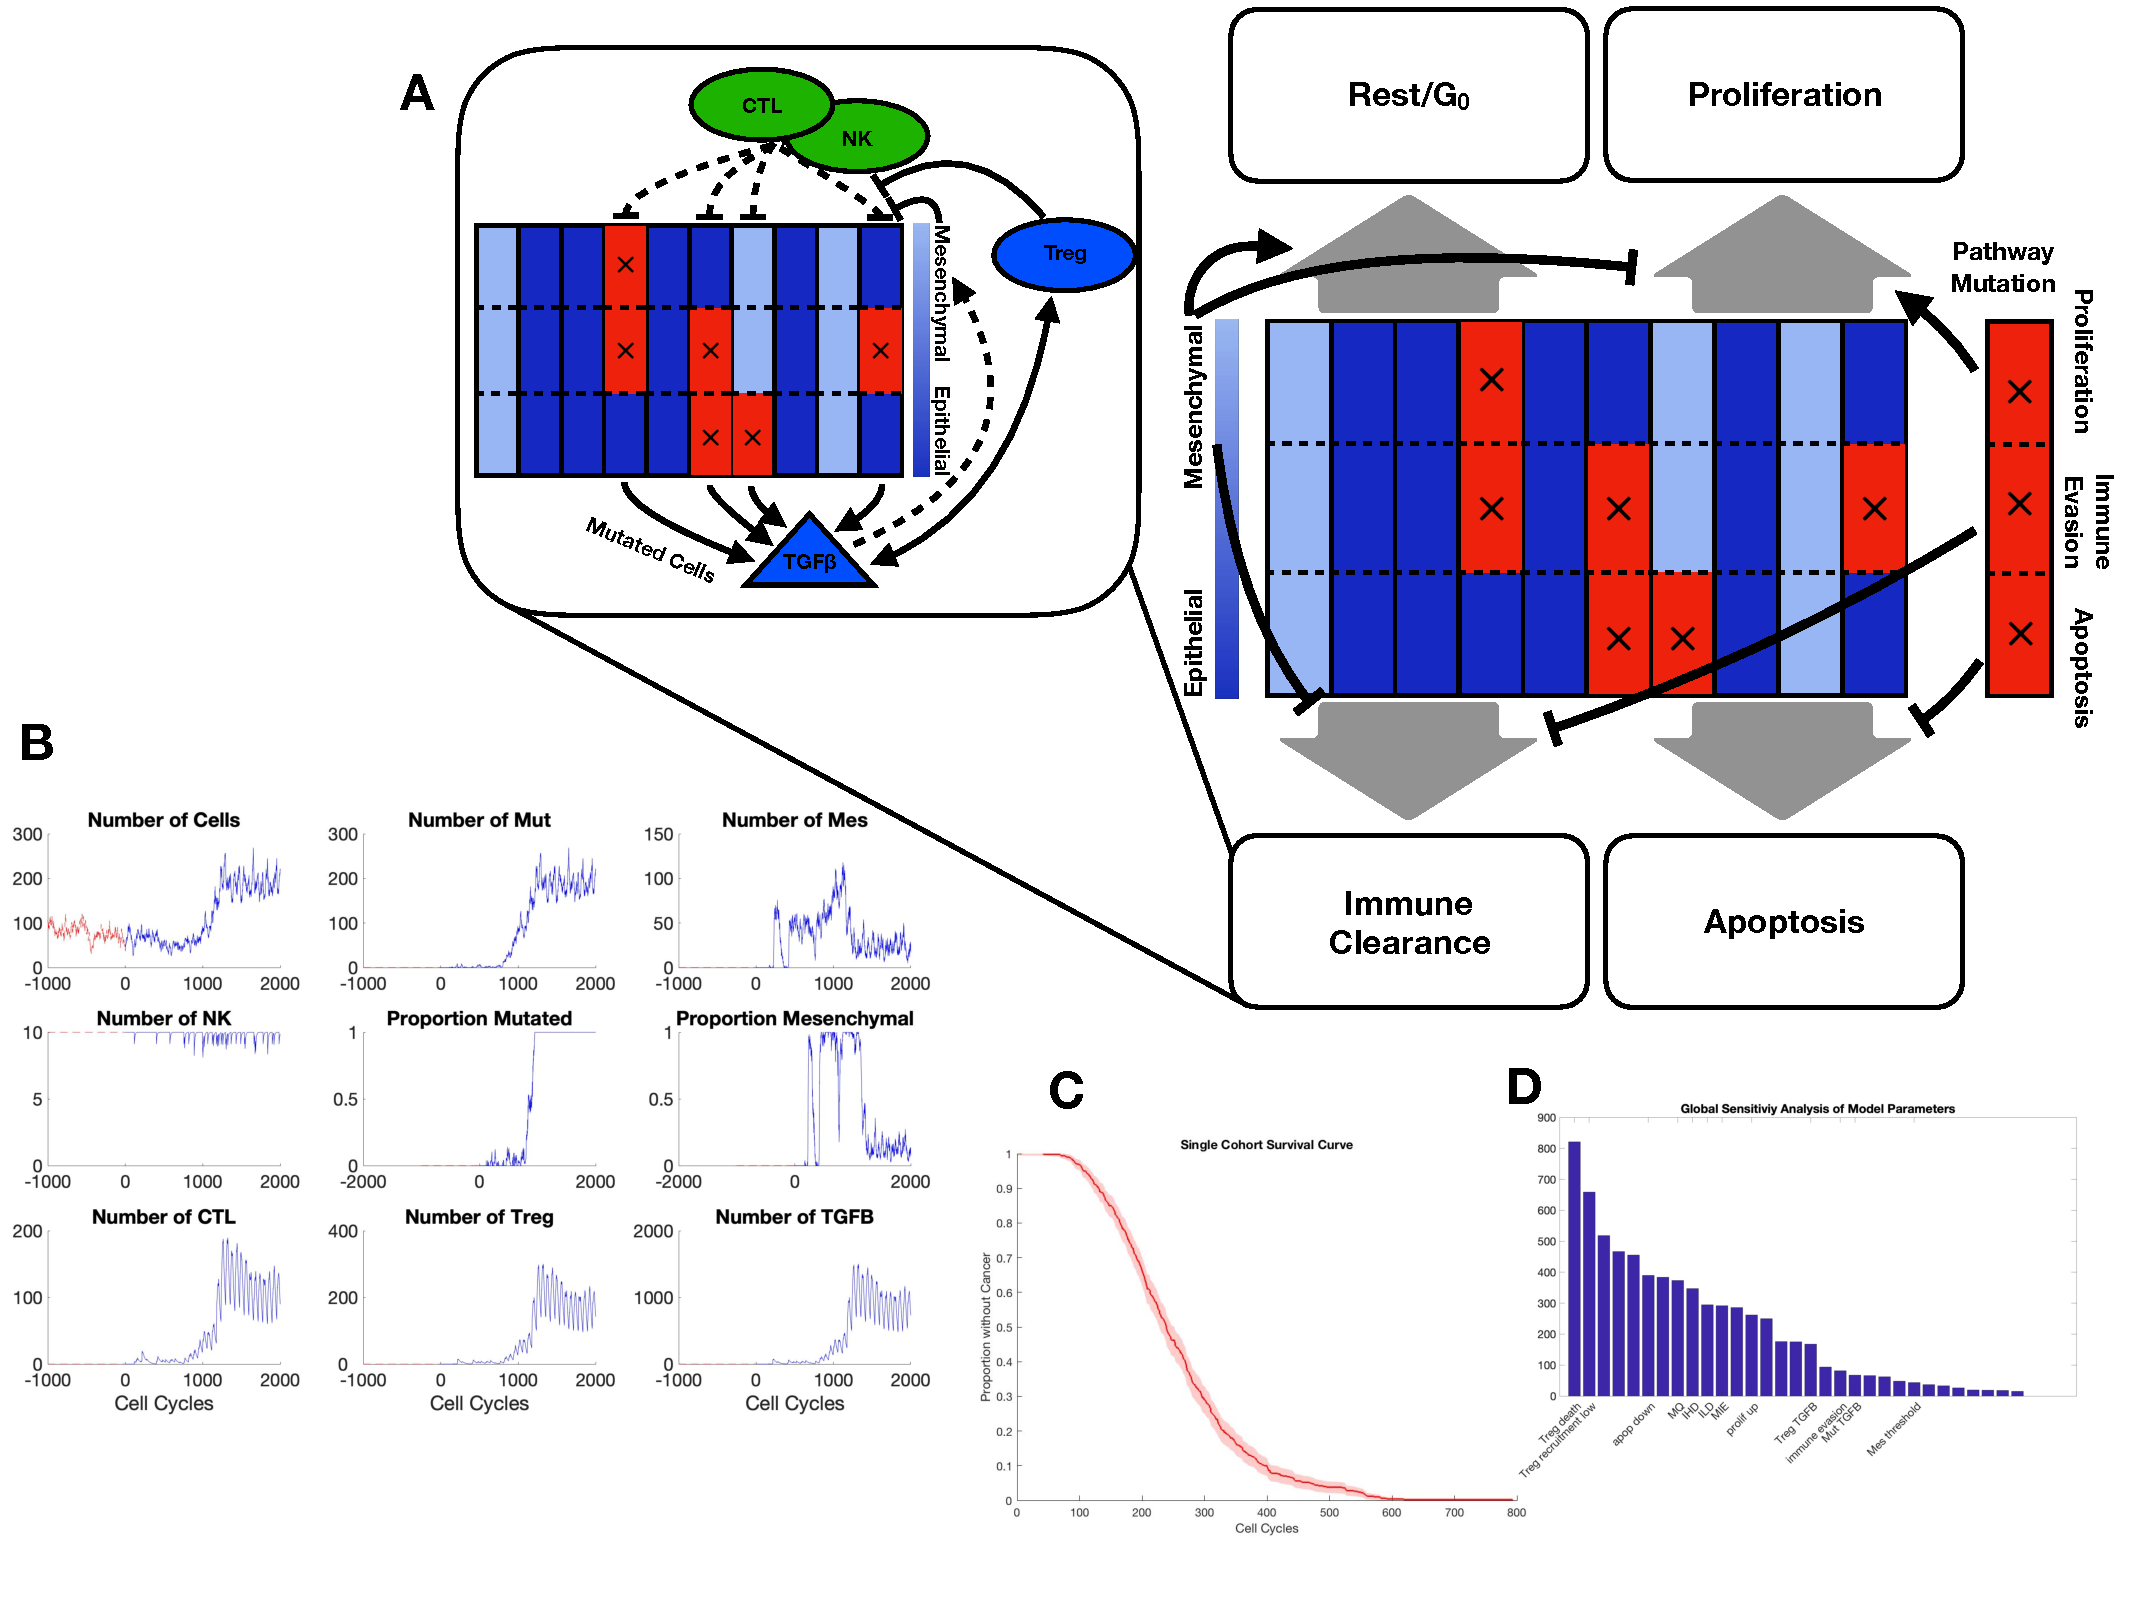
\includegraphics[width=0.9\textwidth]{Figure1/Figure1.pdf}}
\caption{{\bf A.} Schematic depiction of agent-based model components; each of the 10 columns represents a single tumor cell divided into three compartments representing the state (altered or not) of the three pathways with mutagenic potential; red/blue denotes altered/unaltered pathways. Black arrows depict regulation of the cell fate in each cell cycle. Inset depicts major interactions between the immune system and tumor cells.
{\bf B.} A representative simulation of one patient. The model parameter values used can be found in Table S2. 
The inflammation cycling scheme is represented above the patient dynamics. The vertical dashed line denotes the end of the warmup period. Mut: malignant cells; Mes: mesenchymal cells. 
{\bf C.} Survival curve for one cohort of patients with the parameter values given in Table S2.}
\label{fig:ModelIntro}
\end{figure}

We begin by investigating general features of the model to establish baseline conditions and assess the impact of different model components on the key measured outcomes: the probability of progression, and the time to invasion. 
Within the cell cycle, cell fate is determined by rules that are influenced by EMT and immune interactions (Fig. \ref{fig:ModelIntro}A), e.g. if a cell undergoes EMT, its probability of proliferation is reduced; if it gains a  mutation in the apoptosis pathway, its probability of apoptosis is reduced. Meanwhile, NK cells and CTLs attempt to clear malignant tumor cells, and deactivate upon successful tumor cell clearance; Tregs inhibit this cytotoxic activity (\ref{fig:ModelIntro}A Inset).
%Tregs also release TGF-$\beta$ which promotes the recruitment of Tregs, as well as increasing the rate of EMT.
\par
The inflammation cycling scheme for a typical {\it in silico} patient consists of alternating high and low regimes with corresponding effects on the cell populations (Fig. \ref{fig:ModelIntro}B).
For this patient, after warmup, mutations are observed at a rate low enough that they are cleared by cytotoxic cells for about 700 cell cycles, after which the mutated and thus invasive cell population begins to grow, leading to large recruitment of CTLs and Tregs and a peak in the concentration of TGF-$\beta$.
After 841 cell cycles, the proportion of invasive cells reaches 50\%: the threshold defining progression, thus this patient has a time to invasion of 841 cell cycles, or 631 days. Beyond this timepoint, we see a rapid increase in the number of invasive cells until it comprises 100\% of the tumor population. Interesting EMT dynamics are also observed, the proportion of MTCs peaks shortly after the tumor becomes invasive, subsequently the majority of cells transition back to an epithelial state. We observe that while the NK population varies little over the simulation, CTLs and Tregs both undergo large expansions. CTLs and Tregs also appear to oscillate, however note that this is a direct result of the inflammation state, and is not immune cell-intrinsic.

%Considering the immune system dynamics, we see that the NK population is approximately constant, while the adaptive populations (CTL and Treg cells) grow quickly and dwarf NK cells in number following the accumulation of driver mutations.
%The adaptive immune populations also appear to exhibit oscillatory behavior, however note that this is not due to intrinsic dynamics but rather due to the inflammation scheme that the patient is undergoing: alternating between 30 cell cycles of high inflammation and 30 cell cycles of low inflammation. Within each of these periods, adaptive immune populations increase or decrease rapidly in accordance with the inflammation state.
\par 
In order to quantify patient dynamics and invasion-free survival as a population level, we simulate large cohorts of patients similar to the single patient shown in  Fig. \ref{fig:ModelIntro}B. For a cohort of $500$ patients, we simulate survival curves and see that a large number progress quickly to form invasive tumors, whereas a few lie in the tail of the distribution after the mutagenic event that a large number of tumors quickly progress while others takes some time before progressing Fig. \ref{fig:ModelIntro}C. By approximately 1200 cell cycles (2.5 years), all tumors have become invasive..



%we see that all the patients survive for approximately 100 cell cycles (75 days). Subsequently, in the approximate range of $T= [100,300]$, the cancer onset rate is roughly constant, and after $600$ cell cycles, no patients remain cancer free.


\subsection{Identification of key model parameters via global sensitivity analysis}\label{SensAnalysis}
Exploring the parameter spaces of systems biology models {\em adequately} is -- in general -- a hard problem. Fitting parameters via (Bayesian) parameter inference is advisable wherever possible \cite{kirk13_model}. Here, despite a wealth of data on tumor growth dynamics, a lack of sufficient molecular measurements (i.e. immune cell dynamics) precludes inference of the full model. In addition, while inference schemes for agent-based models are developing \cite{gallaher17_hybrid, warne19_simulation}, simulation times remain a hurdle \cite{lambert18_bayesian}. Parameters for some components of the model studied previously can be constrained \cite{guo17_multiscale}. However, even here, new biological processes in the current system could push the model into new behavioral regimes. Thus to sample and characterize the parameter space of the model we use sensitivity analysis.   
\par
The results of Morris one-step-at-a-time sensitivity analysis on the 31 model parameters (Fig. \ref{fig:MOAT}) find a subset of parameters with much higher levels of sensitivity than others. The two most influential by this analysis are the recruitment rates of Tregs and CTLs in the low inflammation state. The parameters influencing EMT are also identified as influencing model outcomes. Since one goal of our analysis is to assess the specific effects of EMT on immune-cancer dynamics, parameters MIE and MGA are of particular interest.
In addition, inflammation parameters controlling the periodic high/low inflammation states are of interest because they strongly influence model outcomes and are capable of being targeted by therapeutic treatments. For immune cell dynamics, the secretion of TGF-$\beta$ by Tregs is found to be sensitive and thus will also be studied further below.


%To assess the sensitivity of the model parameters and thus identify those that are most important in determining progression-free survival times, we performed Morris one-step-at-a-time (OAT) sensitivity analysis (see Methods). 
%The two most influential according to this analysis are the death rate and the recruitment rate of Treg cells, this is most likely due to the dual roles Treg cells play in both suppressing the cytotoxic effects of other immune cells and secreting TGF-$\beta$, which drives EMT.
%This ties Treg cells to all three components of the model.
%Since we seek to separate the effects of different model components, we do not choose the parameters influencing Treg cells for detailed analysis below.


%%%%%%%%%%%%%%%%%%%%%%%%%%%%%%%%%%%%%%%%%%%%%%%%%%%%%%%%
%%%%% PUT THIS SOMEWHERE ELSE  - Supplemental methods ? 
%%%%%%%%%%%%%%%%%%%%%%%%%%%%%%%%%%%%%%%%%%%%%%%%%%%%%%%%
%Many parameters in the model change depending on the inflammation state. For the sake of a naming convention, any parameter which includes ``low'' in the name represents the parameter value when inflammation is low. For when the inflammation is high, these ``low'' parameters get scaled by parameters which include ``up'' in the name.
%The ILD and IHD parameters determine the duration of low and high inflammation, respectively. A cell with altered pathways will be affected by the $\Delta_A$, $\Delta_P$, and $\Delta_{\text{IE}}$ parameters, depending on whether the apoptosis, proliferation, or immune evasion pathways are altered.
%The mesenchymal cells are influenced by the MGA and MIE parameters.
%Finally, $\sigma$, $k_\text{EMT}$, $\tau_\text{max}$, and $K_3$ all control how cells transition between the epithelial and mesenchymal states.



\begin{figure}
\center
{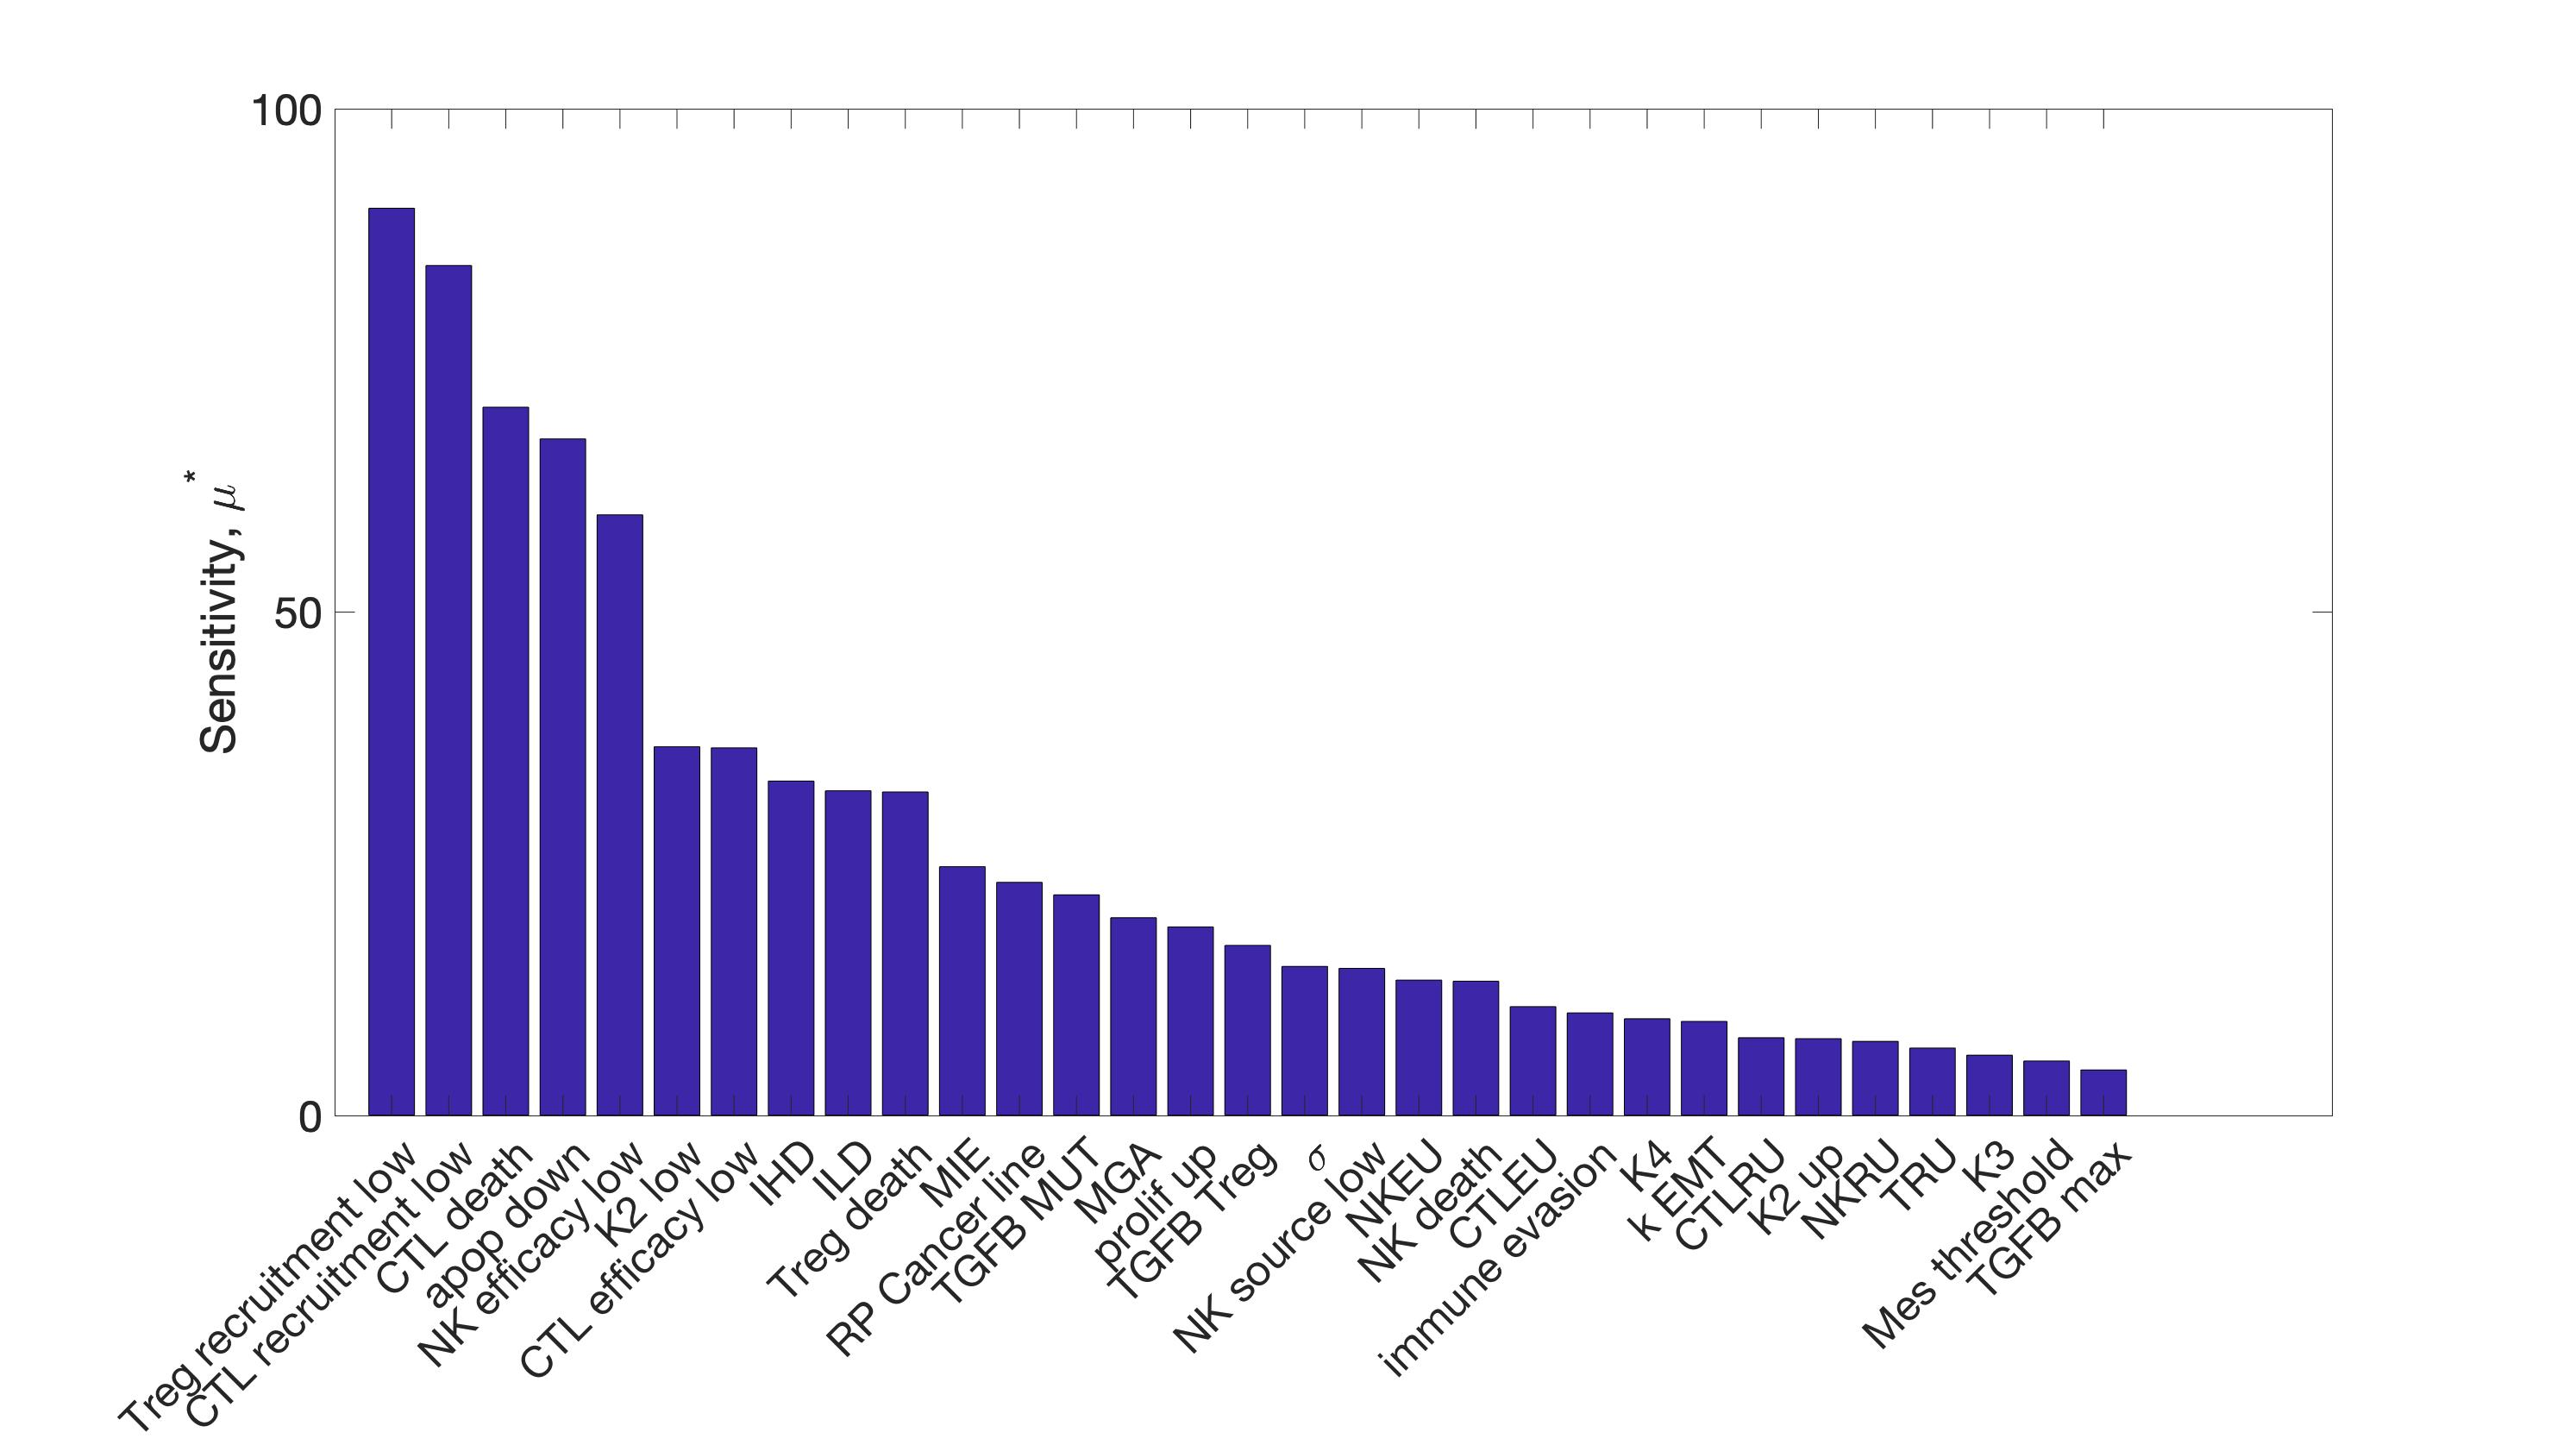
\includegraphics[width=0.85\textwidth]{Figure2/MOAT.jpg}}
\caption{Global sensitivity analysis of model parameters. The sensitivity ($\mu^*$) denotes the average absolute change in the time to invasion over the range of variation of the parameter.}
\label{fig:MOAT}
\end{figure}

\subsection{Mesenchymal properties dramatically alter invasion-free survival times}\label{MesPars}

\begin{figure}
\center
{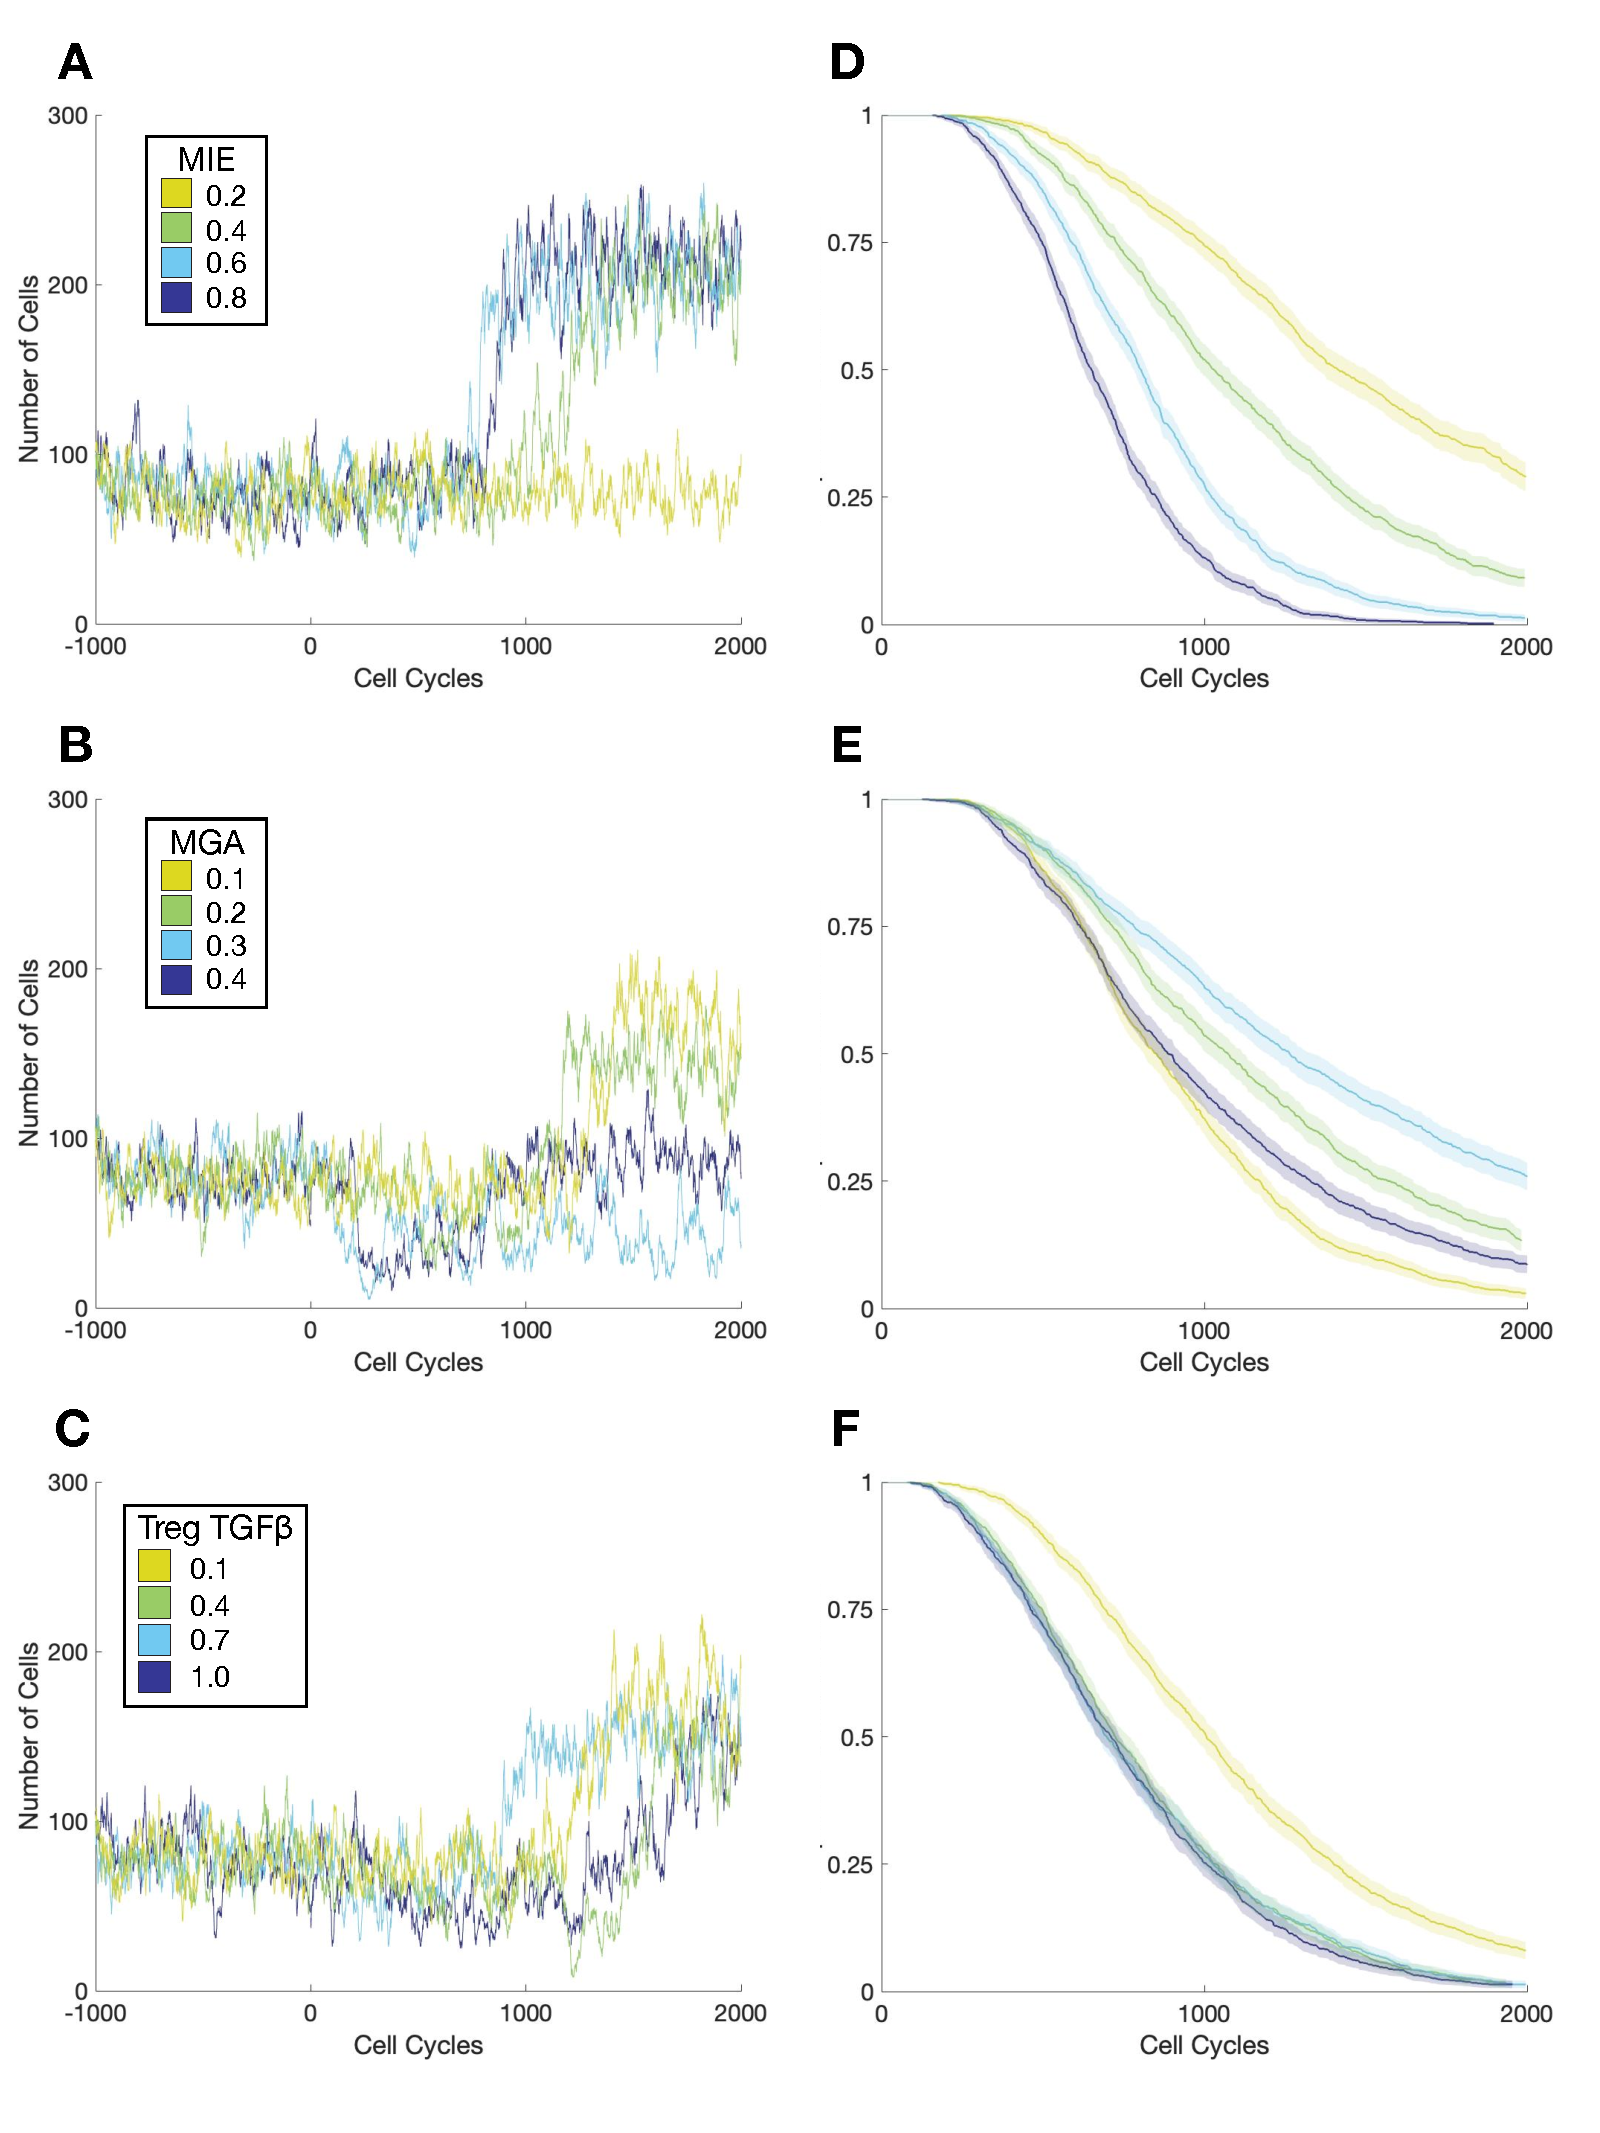
\includegraphics[width=0.85\textwidth]{Figure3/Figure3.pdf}}
\caption{Effects of mesenchymal tumor cell properties on the time to invasion. Trajectories of one patient per cohort including warmup and 2000 cell cycles for {\bf A.} mesenchymal immune evasion (MIE); {\bf A.} mesenchymal growth arrest (MGA); {\bf C.} Production of TGF-$\beta$ by Tregs.
{\bf D.} Survival curve corresponding to changes in the parameter MIE (A) for a patient cohort of 1000. Shaded region represents the 95\% confidence interval over the cohort. 
{\bf E.} Survival curve corresponding to changes in MGA.
{\bf F.} Survival curve corresponding to changes in Treg production of TGF-$\beta$. }
\label{fig:FirstSurvivalCurves}
\end{figure}


Mesenchymal tumor cells (MTCs) are characterized by changes in two parameters: mesenchymal immune evasion (MIE) and mesenchymal growth arrest (MGA). Here we assess the effects of each, alongside the effects of TGF-$\beta$ through its production by Tregs.  
%Both parameters are defined proportionally and hence lie in $[0,1]$, where higher values indicate more mesenchymal-like properties.
% $\Delta_\text{MIE}$ quantifies the reduction in probability that a mesenchymal cell will be subject to immune clearance.
% $\Delta_\text{MGA}$ quantifies the reduction in probability that a mesenchymal cell will proliferate, and is equivalent (in terms of its impact on the cell cycle) to an increased time spent in $G_0$.
%The cytokine TGF-$\beta$ is also involved in the EMT process (by increasing the probability of EMT). All three of these parameters were found to have large effects on the model by the Morris OAT analysis presented in Section \ref{SensAnalysis}. 
As MIE increases, the invasion-free survival decreases (Fig. \ref{fig:FirstSurvivalCurves}A) for all sets of parameters studied: as the subpopulation of invasive cells becomes more resistant to immune clearance, the tumor as a whole grows more resilient and thus can grow faster (Fig. \ref{fig:FirstSurvivalCurves}D).
\par
The relationship between MGA and invasion-free survival times displays a very different trend, and is non-monotonic with a local maximum appearing. For small values of MGA, increasing the MGA parameter results in increasing the invasion-free survival (Fig \ref{fig:FirstSurvivalCurves}B, E). However for large values of MGA, invasion-free survival times decrease. This is explored further below.
%This result is explored in Section \ref{KeyEMT}.
%As MGA increases, invasion-free survival increases: lower proliferation rates for mesenchymal cells slow down cancer progression (Fig \ref{fig:FirstSurvivalCurves}B).
%This is not intuitive, since decreased proliferation rates affects all mesenchymal cells, not just the invasive cells.
\par
TGF-$\beta$ varies according to its production by tumor cells and its production by Tregs. Here we assess the effects of varying the production of  TGF-$\beta$ by Tregs on invasion-free survival (Fig \ref{fig:FirstSurvivalCurves}B, E). We find, interestingly, that at lower production rates of TGF-$\beta$ lead to more rapid invasion or if it survives to a certain time point, a longer time to invasion.

%The effect we do see is that lower Treg TGF-$\beta$ results in more rapid invasion or if it survives to a certain time point, a longer time to invasion.
%Here, we choose to focus on the results of the effect of MIE and MGA as the more direct link to the mesenchymal phenotype.



\subsection{A key EMT regime maximizes cancer-free survival time under chronic inflammation}\label{KeyEMT}

\begin{figure}
\center
{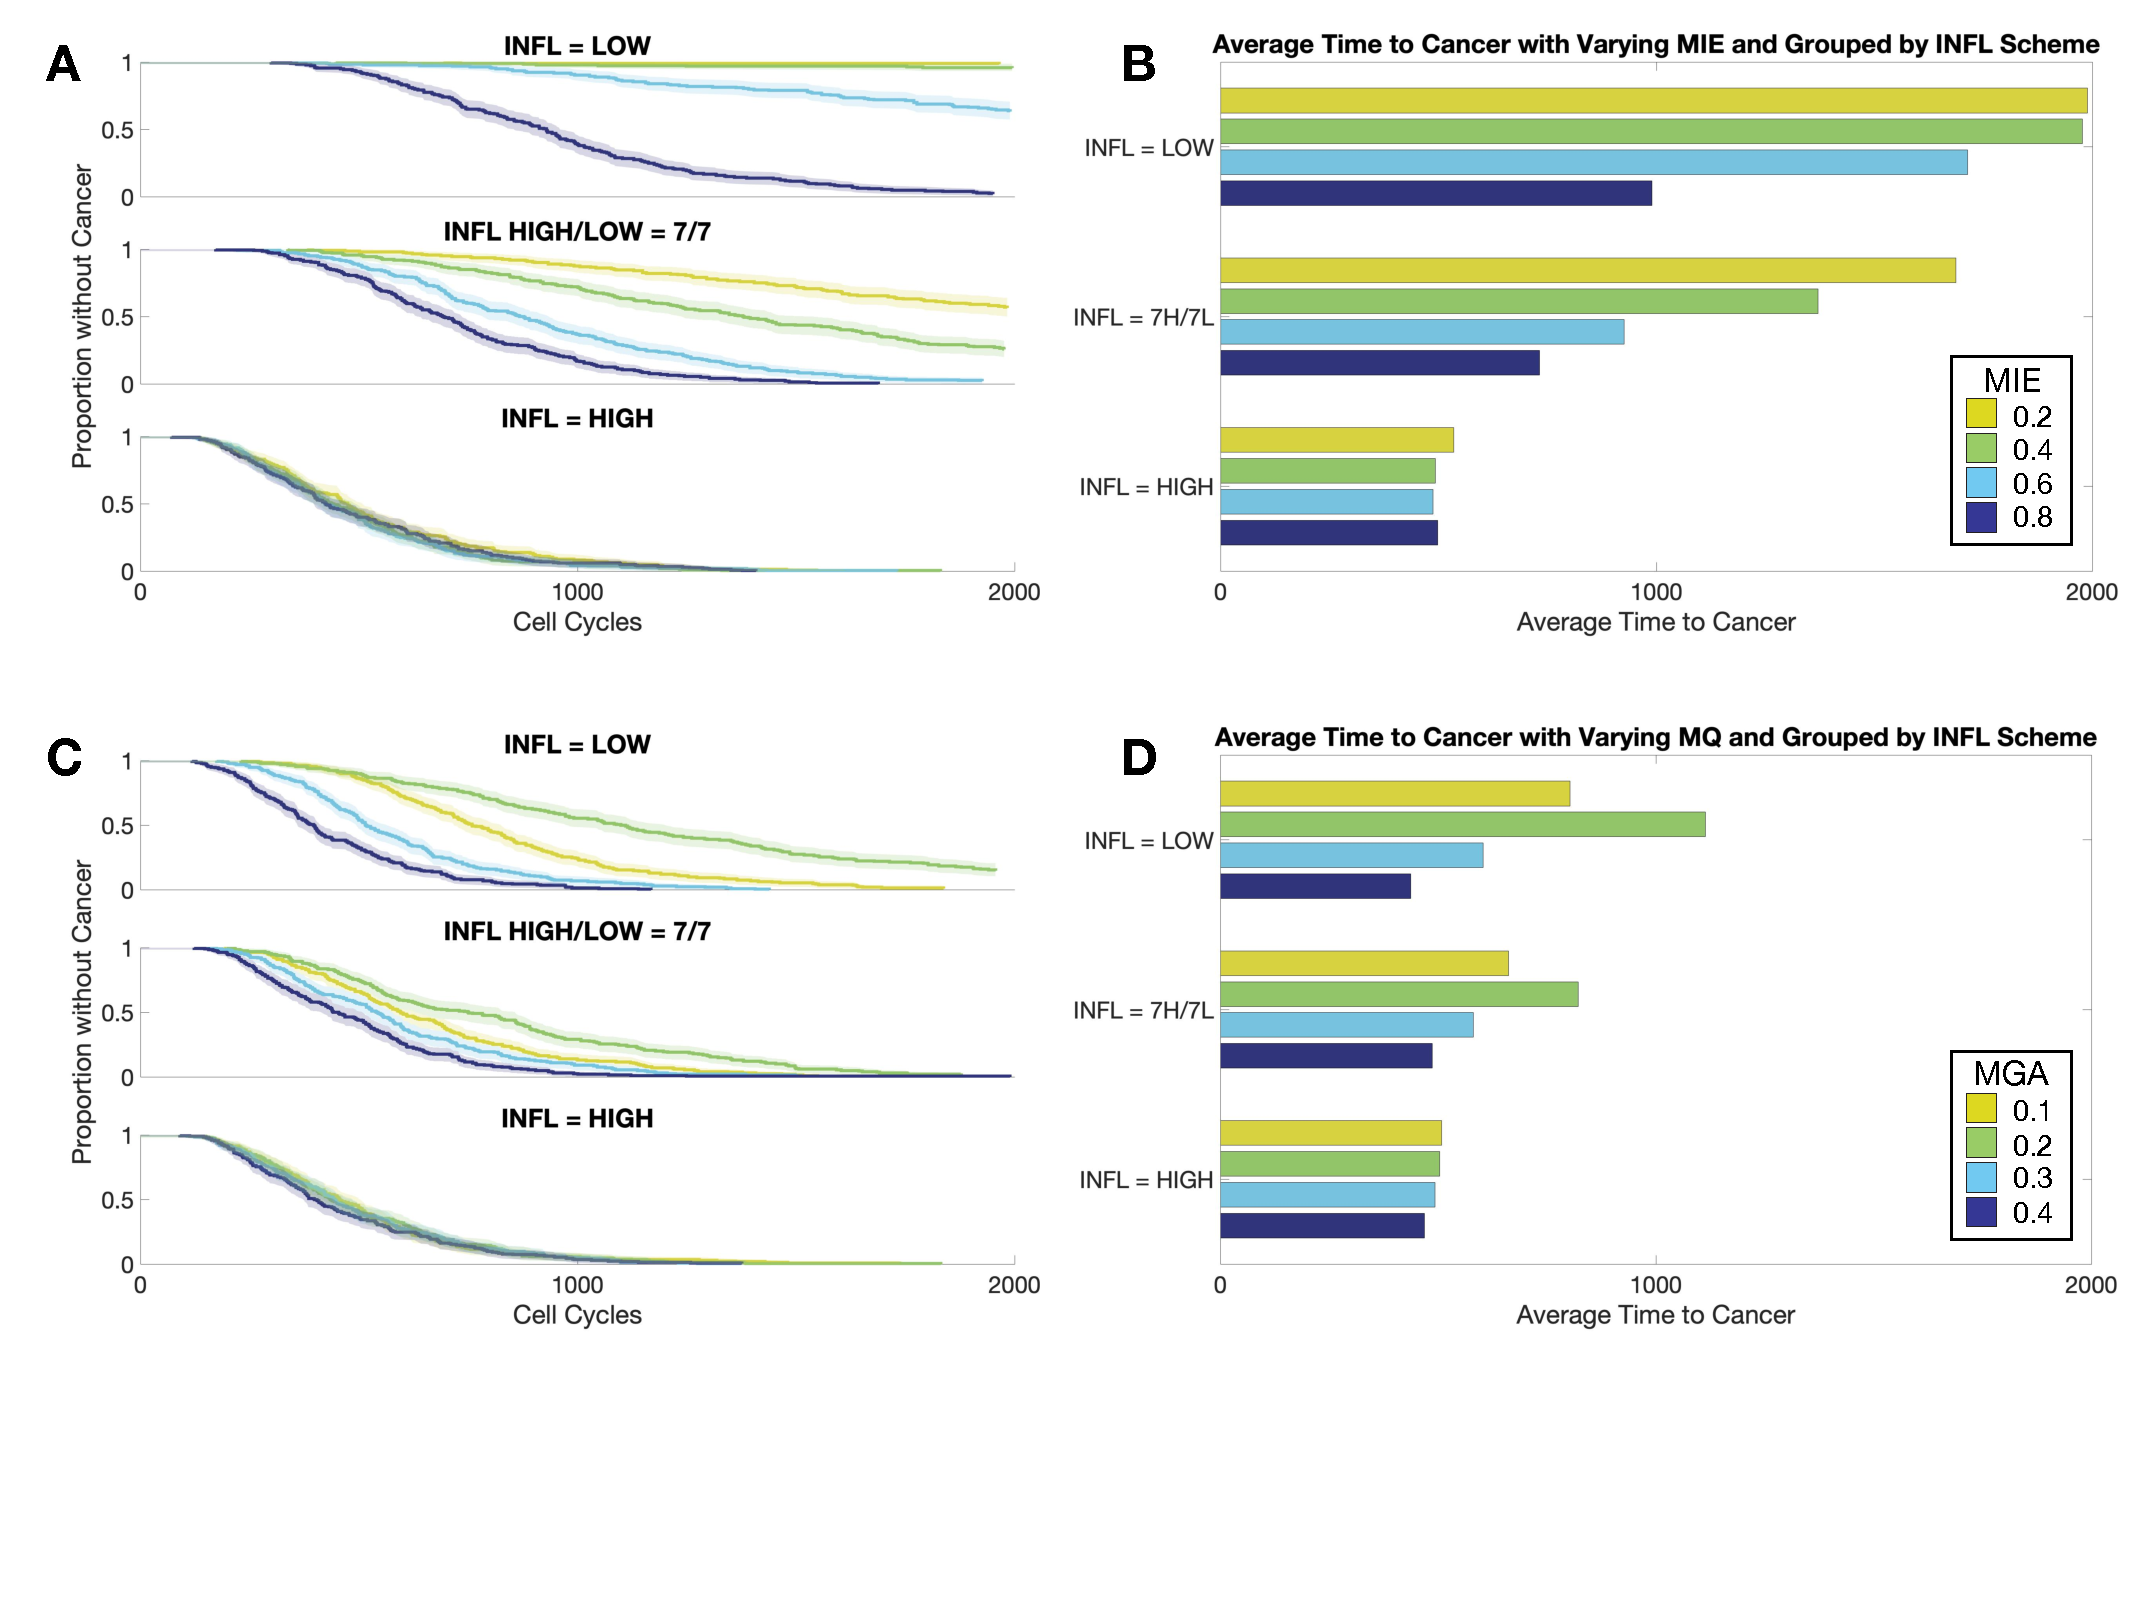
\includegraphics[width=0.95\textwidth]{Figure4/Figure4.pdf}}
\caption{Effects of inflammation on the time to invasion under different cycling schemes. {\bf A-B.} As MIE varies, survival curves (each of 200 patients)  and corresponding bar plots to summarize the mean Time to Cancer for each cohort are shown. {\bf C-D.} As MGA varies, survival curves  and corresponding bar plots to summarize the mean Time to Cancer for each cohort are shown.}
\label{fig:VaryINFL_and_MesPars}
\end{figure}


To investigate how competing interactions within the inflammatory tumor microenvironment affect EMT, we explored the effects of varying inflammation on invasion-free survival. Patient cohorts were simulated under different inflammation regimes: permanently low inflammation; permanently high inflammation; or variable (periodic high/low) inflammation. 
Compared to the other inflammation states, permanently high inflammation results in outcomes that vary more subtly with changes in the mesenchymal parameters (Fig. \ref{fig:VaryINFL_and_MesPars}).
When the inflammation state is either permanently or temporarily low, surprising trends emerge. In both these cases, invasion-free survival time is negatively correlated with MIE, and a local maximum for the invasion-free survival time is found with respect to MGA (close to $\Delta_\text{MGA}= 0.2$).

%For patients drawn from cohorts in a permanently high inflammatory state, the relationship between mesenchymal parameters and invasion-free survival is monotonic, i.e. increasing either MIE (Fig. \ref{fig:VaryINFL_and_MesPars}A-B) or MGA (Fig. \ref{fig:VaryINFL_and_MesPars}C-D) decreases the invasion-free survival time.
%However, under regimes with either temporary or permanent periods of low inflammation, different relationships emerge: a local maximum for the invasion-free survival time is found with respect to MGA ($\Delta_\text{MGA}= 0.3$). This is seen both for intermittent or low inflammation (Fig. \ref{fig:VaryINFL_and_MesPars}D). 

\par
These differences in the mean invasion-free survival lead to striking variation in outcomes: tumors can be contained in situ for up to twice as long as they would otherwise be simply by varying the rates of mesenchymal growth arrest. These predictions point to intriguing therapeutic outcomes: a patient suffering intermittent high inflammatory attacks will benefit directly from EMT-directed therapies, however patients for whom a relatively high inflammation state is observed continuously will not obtain this benefit.
\par
When MIE is varied under different inflammation cycling schemes, for all the periodic inflammation schemes studied, increasing MIE will decrease the invasion-free survival (i.e. worsen cancer progression and prognosis)  (Fig. \ref{fig:VaryINFL_and_MesPars}B). In the case of continuously high inflammation, the effects of MIE are minimal. Thus, under any inflammation regime with periods of low inflammation, as we might intuitively assume, any reduction in mesenchymal immune evasion will lead to improvements in patient outcomes.


\subsection{Analysis of data from TCGA supports model predictions: EMT phenotypic properties worsen patient outcomes}\label{tcga}

\begin{figure}
\center
{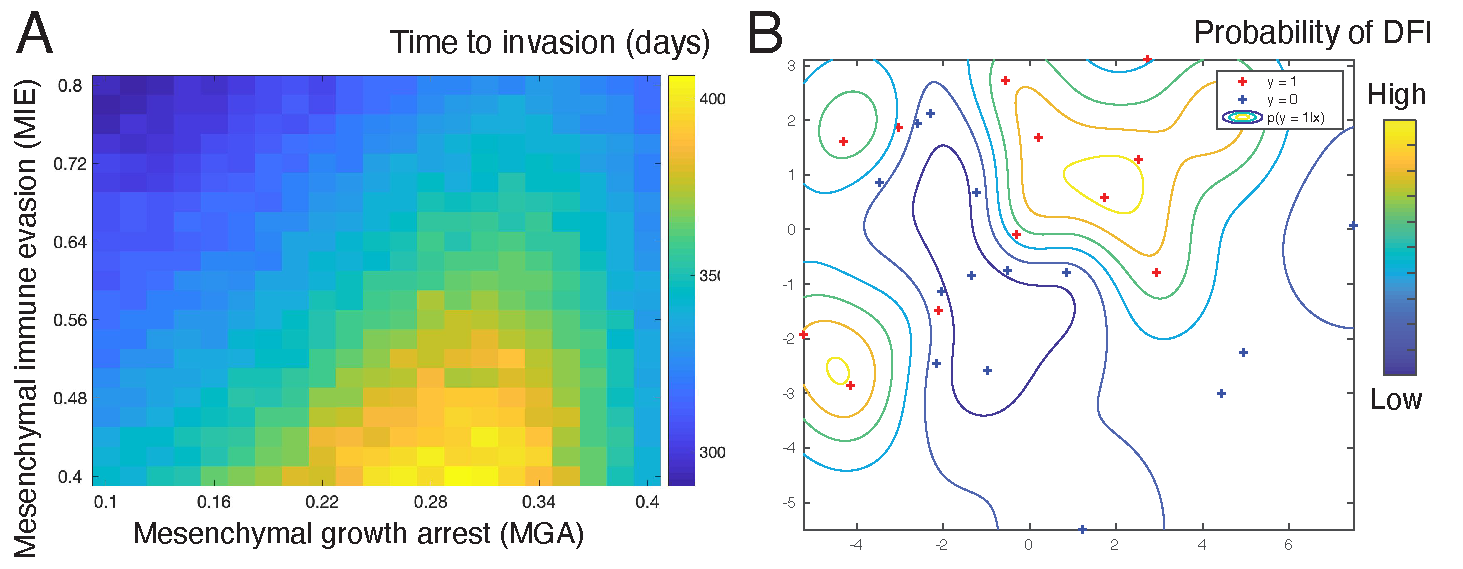
\includegraphics[width=0.85\textwidth]{Figure5/FigHeatmapLIHC.pdf}}
\caption{{\bf A.} Summary of the effects of MIE and MGA on invasion-free survival.
  {\bf B.} Bayesian classification model applied to liver hepatocellular carcinoma (LIHC). Patients projected into 2D by principle components analysis to determine most probable regions of disease-free interval (DFI). Two local maxima are identified, separated by \tcr{XXXX}.
}
\label{fig:MIEvsMGA}
\end{figure}


\begin{figure}
\center
{\includegraphics[width=0.65\textwidth]{Figure6/OV.pdf}}
\caption{A. K-means clustering of OV using gene ontology terms indicative of EMT and inflammation signatures ($k=2$).
B. Survival plots corresponding to the clustering on EMT and inflammation.
C. K-means clustering of OV using gene ontology terms indicative of an EMT signature ($k=2$).
D. Survival plots corresponding to the clustering on EMT.
E. K-means clustering of OV using gene ontology terms indicative of inflammation ($k=2$).
F. Survival plots corresponding to the clustering on inflammation.}
\label{fig:OV}
\end{figure}

%The effects that mesenchymal phenotypic properties have on progression can also be assessed by studying mesenchymal immune evasion ($\Delta_\text{MIE}$) and mesenchymal growth arrest ($\Delta_\text{MGA}$) on a heatmap (Fig. \ref{fig:MIEvsMGA}). We found that over the full range of values of $\Delta_\text{MGA}$ considered, increasing $\Delta_\text{MIE}$ decreases the invasion-free survival time.


\par
To compare these model predictions with experimental studies, we analyzed data from The Cancer Genome Atlas (TCGA) \cite{Weinstein}. We studied the effects of immune interactions and EMT on cancer prognosis, especially on tumors for which inflammation is known to play an important role, such as those of the colon, or pancreas, or liver  \cite{greten2019inflammation,hu2010inflammation}.
The TCGA Pan-Cancer Clinical Data Resource provides multiple computed clinical endpoints for pancreatic cancer (PAAD) \cite{liu2018integrated}.
Here, we focus on the disease-free interval (DFI) and the overall survival (OS). A tumor with a short DFI will likely undergo rapid progression post-treatment. We thus expect the distance between DFI and OS to be small for a rapidly progressing tumor, following initial detection. We can therefore characterize tumors as either rapidly progressing or slowly progressing by defining a threshold for the ratio DFI/OS. We selected tumors for which Clinical Data Resource profiles indicated slow progression (ovarian, OV; skin cutaneous melanoma, SKCM; liver hepatocellular carcinoma, LIHC) and two tumors whose profiles indicated rapid progression (pancreatic cancer, PAAD; lung adenocarcinoma, LUAD).
\par
The effects on cancer progression of mesenchymal phenotypic properties predicted by the model are summarized in Fig. \ref{fig:MIEvsMGA}A. Where, %For all values of MGA, increasing MIE leads to a decrease in invasion-free survival times.
for a given value of MIE, there is an optimal value of MGA that maximizes invasion-free survival. %Moreover, this optimum increases with increasing MIE.
We use two models to compare these predictions with TCGA data: a Bayesian supervised classification model, and survival analysis with k-means clustering (see Methods). The classification model applied to liver carcinoma identifies local maxima that promote survival, demonstrating intriguing similarities with model results (Fig.  \ref{fig:MIEvsMGA}B). \tcr{Classification plots for OV/PAAD in SI}
\par
For each cohort of patients for which we have clinical and expression data, we cluster the patients via k-means (n = 2) against gene ontologies relating to either: EMT signature alone, inflammatory signature alone, or the combination of both signatures. We then plot the corresponding survival curves (using the OS from TCGA) for each of the two groups (Fig.  \ref{fig:OV} for ovarian cancer and Fig. \ref{fig:PAAD} for pancreatic cancer).
%(Figures \ref{fig:OV}C, \ref{fig:PAAD}C), only inflammation (Figures \ref{fig:OV}E, \ref{fig:PAAD}E), and both EMT and inflammation (Figures \ref{fig:OV}A, \ref{fig:PAAD}A).
We see that for both these tumor types, survival is affected by the gene ontology signature, and the combination of both EMT and inflammatory signatures has a greater impact on survival than the effects of either EMT or inflammation alone.
This suggests that in considering interactions between cancer and the immune system, is it of critical importance to consider the effects of EMT, as these can significant impact outcomes and should not be overlooked. 
\par
The model considered here studies tumor progression from in situ to invasive disease from a homogeneous initial point, whereas the data address how cancer may progress following treatment, thus comparisons between model and data should be made carefully. Nonetheless the core cellular tumor dynamics are at play
%The comparison between simulation and data here is indirect since the model studies the progression of cancer from an arbitrary starting point, while the data address the progression of cancer following treatment, but analogous processes are at play
 both during the tumor progression addressed by the model, and post-treatment progression described in data from TCGA. Of particular note, the plasticity of tumor cells allows them to evade treatment by undergoing post-treatment processes resembling the de-novo appearance of cancer\cite{sanchez2018slow}.

\begin{figure}
\center
{\includegraphics[width=0.65\textwidth]{Figure6/PAAD.pdf}}
\caption{A. K-means clustering of PAAD using gene ontology terms indicative of EMT and inflammation signatures ($k=2$).
B. Survival plots corresponding to the clustering on EMT and inflammation.
C. K-means clustering of PAAD using gene ontology terms indicative of an EMT signature ($k=2$).
D. Survival plots corresponding to the clustering on EMT.
E. K-means clustering of PAAD using gene ontology terms indicative of inflammation ($k=2$).
F. Survival plots corresponding to the clustering on inflammation.}
\label{fig:PAAD}
\end{figure}




%%%%%%%%%%%%%%%%%%%%%%%
%                      DISCUSSION                       %
%%%%%%%%%%%%%%%%%%%%%%%

\section{Discussion}\label{Discussion}
Despite the intense research focus on interactions between cancer and the immune system, and well as on the effects of EMT on cancer, there has not previously, to the best of our knowledge, been a model developed that combines these three components. Here we studied cancer, the immune system, and EMT, during the progression from an in situ tumor to invasive disease. We saw this as a particularly pressing need given the shared factors influencing all these components, such as TGF-$\beta$. We used an individual cell-based model framework to describe the multiscale processes that can lead to cancer: DNA damage occurs during the cell cycle and this can lead to mutations in pathways that affect cell fitness, which in turn affects the cell population dynamics. Population dynamics are also influenced by the intrinsic state of the cell (through EMT), and extrinsic immune factors.
\par
We found that this model recapitulated invasion-free survival dynamics. Using global parameter sensitivity analysis, we identified parameters exerting key control over model behavior. Focusing on these led us to identify that increasing mesenchymal immune evasion and increasing Treg TGF-$\beta$ production both lead to shorter invasion-free survival times. However, varying the level of inflammation led to paradoxical effects with regards to mesenchymal growth arrest: under regimes with periods of low inflammation, an optimal level of mesenchymal growth arrest can improve outcomes and maximize the invasion-free survival. To test these predictions, we performed unsupervised analysis of pancreatic cancer data from The Cancer Genome Atlas, and looked at survival across groups with {\em rapidly progressing} or {\em slowly progressing}  tumors. We found that combinatorial effects of EMT + inflammation increased the differences in survival between groups.
\par
To capture the essential characteristics of the model, we summarized {\em in silico} patient studies with a single parameter: the invasion-free survival time (see Fig. 1B for a reminder of the full model heterogeneity). There are, of course, many trajectories that result in cancer progression. Analysis of the transient cell dynamics in cancer in situ and during progression is a pressing need to shed insight into cellular biomarkers of cancer.
\par
The predictions of this model offer promising leads in elucidating the competing roles of immune cells and EMT during tumor progression, but much remains to be done. Further development of the inflammation module of this model is important given the large and sometimes paradoxical roles that the inflammatory state exerts on tumor cells and invasion-free survival (Figs. \ref{fig:MOAT} and \ref{fig:VaryINFL_and_MesPars}B, D). Currently, inflammation is modeled as independently cycling between high and low schemes, however several model components contribute to the inflammatory state. This can be modeled for example by assuming that the level of inflammation depends on the number of and the degree of mutations that tumor cells harbor.
%% not sure about
%Another layer of complexity is revealed by the natural anti-inflammatory role of Tregs. One consequence of the current model is that decreasing the number of Tregs increases the cancer-free survival. Clearly, there exists a trade-off to be accounted for, and adding to the model the main effector function of Tregs could remedy this and add depth to our understanding of the various roles that Tregs play in and around the tumor.
The competing roles that TGF-$\beta$ play throughout the tumor and its microenvironment also warrant further investigation. We found that -- below a certain threshold -- reduction of TGF-$\beta$ increases the time to invasion (Fig. \ref{fig:FirstSurvivalCurves}E): reducing  TGF-$\beta$ in the TME can benefit survival. Recent experiment work in support of this demonstrated that TGF-$\beta$ drives tumor suppression in pancreatic cancer by promoting EMT \cite{david16_tgfv}. TGF-$\beta$, however, is implicated in numerous other cellular signaling processes, and changing TGF-$\beta$ concentration even in a local environment could have large off-target effects. Indeed, it has been shown that TGF-$\beta$ promotes invasion and heterogeneity while  suppressing cell proliferation in squamous cell carcinoma \cite{oshimori15_tgfv}. To help account for such complex circuitry, future work should incorporate the effects of signaling factors downstream of TGF-$\beta$ on tumor cell dynamics. We are currently developing a larger TGF-$\beta$ signaling pathway component within the full model that permits crosstalks between ETCs, MTCs, and immune cell populations through transcriptional signaling activity.
\par
Further {\em in silico} work on this model and its extensions will explore (and exploit) the heterogeneity of tumor evolution in greater depth. Tumor heterogeneity greatly enhances the capabilities of the tumor to evade immune effects. Studying the consequences of this increased heterogeneity following disease incidence, i.e. decanalization \cite{gibson09_decanalization}, is too-often sidelined, despite mounting evidence in support of its prominent role in cancer evolution \cite{cyll17_tumour, punt17_tumour, dagogo-jack18_tumour}. Despite these challenges (for which disease complexity is often in part responsible), great progress has been and continues to be made. As we are rapidly approaching a new generation of immunotherapies, it is these very complexities that we must better understand in order to control or eradicate the disease.


\section*{Acknowledgements}
Q.N. would like to acknowledge partial support for this work from National Institutes of Health grants R01GM123731, U01AR073159, and U54-CA217378; National Science Foundation grants DMS1562176 and DMS1763272; Simons Foundation grant (594598); and the Jayne Koskinas Ted Giovanis Foundation for Health and Policy joint with the Breast Cancer Research Foundation. A.L.M. would like to acknowledge partial support for this work from an American Cancer Society grant \#IRG-16-181-57.


\bibliography{mybib,amrefs}
\bibliographystyle{plos2015}

\end{document}
